\documentclass[UTF8]{ctexart}
\usepackage{amsmath, amsthm, amssymb, anyfontsize, bm, float, graphicx,mathrsfs,longtable, subfigure}
\usepackage[hidelinks]{hyperref}
\usepackage{tikz}
\ctexset { section = { format={\Large \bfseries } } }
\newtheorem{theorem}{定理}[section]
\pagestyle{empty}
\begin{document}

\date{}
\maketitle


\begin{figure}[H]
    \centering
    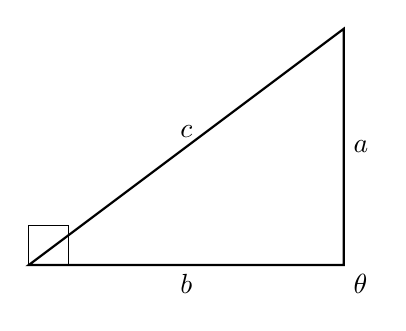
\begin{tikzpicture}
        \draw[thick] (0,0) -- (4,0) -- (4,3) -- cycle;
        \draw (2,0) node[below] {$b$};
        \draw (4,1.5) node[right] {$a$};
        \draw (2,1.5) node[above] {$c$};
        \draw (4,0) node[below right] {$\theta$};
        \draw (0,0) rectangle (0.5,0.5);
    \end{tikzpicture}
    \caption{正割定义示意图}
\end{figure}

\end{document}